%%%%%%%%%%%%%%%%%%%%%%%%%%%%%%%%%%%%%%%%%%%%%%%
%
% Template for Bachelor degrees
% DISI - Dipartimento di Ingegneria e Scienza dell’Informazione
% DISI - Department of Information Engineering and Computer Science
%
% update 2020-08-30
%
% To generate pdf 
% pdflatex __filename__.tex
% bibtex __file_name__.aux
% pdflatex __file_name__.tex
% pdflatex __file_name__.tex
%
%%%%%%%%%%%%%%%%%%%%%%%%%%%%%%%%%%%%%%%%%%%%%%%

% 2 side format
\documentclass[epsfig,a4paper,11pt,titlepage,twoside,openany]{book}
\usepackage{epsfig}
\usepackage{plain}
\usepackage{setspace}
\usepackage[paperheight=29.7cm,paperwidth=21cm,outer=1.5cm,inner=2.5cm,top=2cm,bottom=2cm]{geometry} % layout setting
\usepackage{titlesec} % custom setup title of chanpter
% \usepackage{newtxtext,newtxmath} % times new roman
\usepackage{tabularx}
\usepackage{graphicx}
\usepackage{subcaption}
\usepackage{listings}
\usepackage{booktabs}
% Configuration for the listings package
\lstset{
    basicstyle=\ttfamily\small,
    frame=single,                     % adds a frame around the code
    numbers=left,                     % line numbers on the left
    numberstyle=\tiny,                % make line numbers tiny
    tabsize=4,                        % set tab space width
    breaklines=true,                  % break too long lines
    keywordstyle=\bfseries,           % style for keywords (if, for, etc.)
    columns=fullflexible
}

%%%%%%%%%%%%%%
% support for accented letters
%
%\usepackage[latin1]{inputenc} % Windows;
\usepackage[utf8]{inputenc} % Linux (unicode package is required);
%\usepackage[applemac]{inputenc} % Mac.

\singlespacing

% italian language
%\usepackage[italian]{babel}
\usepackage[hidelinks]{hyperref}
\begin{document}

  % no page number
  \pagenumbering{gobble} 
  \pagestyle{plain}

\thispagestyle{empty}

\begin{center}
  \begin{figure}[h!]
    \centerline{
\psfig{file=marchio_unitrento_colore_it_202002.eps,width=0.6\textwidth}}
  \end{figure}

  \vspace{2 cm} 

  \LARGE{Department of Information Engineering and Computer Science\\}

  \vspace{1 cm} 
  \Large{Bachelor's Degree in\\
    Computer Science
    % Computer Science
    % Computer, Communication and Electronic Engineering
    % Information and Communications Engineering
    % Information and Business Organization Engineering
    % Electornics and Telecommunications Engineerign
  }

  \vspace{2 cm} 
  \Large\textsc{Final Dissertation\\} 
  \vspace{1 cm} 
  \Huge\textsc{Distributed Machine Learning Self-Learning Pipeline for Edge Sensing Applications\\}
  \Large{\it{Implementing Distributed Machine Learning Techniques on Resource-Constrained Devices: A Study with the Spark SR1020 UWB Family Evaluation Kits.}}


  \vspace{2 cm} 
  \begin{tabular*}{\textwidth}{ c @{\extracolsep{\fill}} c }
  \Large{Supervisor} & \Large{Student}\\
  \Large{Kasim Sinan Yildirim}& \Large{Daniele Stella}\\
  \end{tabular*}

  \vspace{2 cm} 

  \Large{Academic year 2022/2023}
  
\end{center}



  %\clearpage
  \newpage
\null
\newpage
 
%%%%%%%%%%%%%%%%%%%%%%%%%%%%%%%%%%%%%%%%%%%%%%%%%%%%%%%%%%%%%%%%%%%%%%%%%%
%%%%%%%%%%%%%%%%%%%%%%%%%%%%%%%%%%%%%%%%%%%%%%%%%%%%%%%%%%%%%%%%%%%%%%%%%%
%% Note
%%%%%%%%%%%%%%%%%%%%%%%%%%%%%%%%%%%%%%%%%%%%%%%%%%%%%%%%%%%%%%%%%%%%%%%%%%
%% Thanks/ Acknowledgements section is optional
%%%%%%%%%%%%%%%%%%%%%%%%%%%%%%%%%%%%%%%%%%%%%%%%%%%%%%%%%%%%%%%%%%%%%%%%%%
%%%%%%%%%%%%%%%%%%%%%%%%%%%%%%%%%%%%%%%%%%%%%%%%%%%%%%%%%%%%%%%%%%%%%%%%%%
  \thispagestyle{empty}

\begin{center}
  {\bf \Huge Acknowledgements}
\end{center}

\vspace{4cm}


%\textit{
\emph{
I would like to extend my profound gratitude to my supervisor, Prof. Kasim Sinan Yildirim, for his unwavering guidance, expertise, and encouragement throughout the course of my research. His insights have been pivotal in shaping the trajectory of my work.}
\emph{My appreciation further extends to Prof. Gian Pietro Picco, Dr. Davide Vecchia, and Dr. Matteo Trobinger. Their insightful discussions, suggestions, and feedback have undoubtedly enriched my understanding and inspired me to explore new avenues.}
\emph{I also wish to convey my heartfelt thanks to Christian Sassi, Davide Molteni, the University of Trento, and everyone else who provided invaluable support, creating an environment that championed both teamwork and individual academic pursuits.}

\emph{My research journey also involved collaborative efforts with Christian Sassi. As research interns at the University of Trento, Christian and I jointly undertook the comprehensive characterization of the Spark SR1020 Ultra-Wideband (UWB) radios, examining their performance metrics in depth. In light of this collaboration, and in the spirit of academic integrity and transparency, we wish to highlight the following:
}
%}
\begin{itemize}
    \item \textit{Our combined efforts are reflected in shared content, including but not limited to testing protocols, environmental conditions, empirical data, and initial conclusions.}
    \item \textit{Despite this shared foundation, our respective theses stand as distinct and independent works, each with its unique research focus. While I, Daniele Stella, explore the intricacies of power consumption, Christian zeroes in on latency testing and data rate evaluations. Our shared test results from the range evaluation are approached differently in line with our individual research objectives.}
    \item \textit{We have ensured that all overlapping content is aptly credited and referenced, acknowledging our collaborative endeavors.}
\end{itemize}


  \clearpage
  \pagestyle{plain} % no heading, footer with centered page number

  
  % page number with Arabic format
  \mainmatter

%%%%%%%%%%%%%%%%%%%%%%%%%%%%%%%%%%%%%%%%%%%%%%%%%%%%%%%%%%%%%%%%%%%%%%%%%%
%%%%%%%%%%%%%%%%%%%%%%%%%%%%%%%%%%%%%%%%%%%%%%%%%%%%%%%%%%%%%%%%%%%%%%%%%%
%% Note
%%%%%%%%%%%%%%%%%%%%%%%%%%%%%%%%%%%%%%%%%%%%%%%%%%%%%%%%%%%%%%%%%%%%%%%%%%
%% The maximum number of pages is 30, including:
%%   index
%%   abstract
%%   chapters
%% Excluding:
%%   frontispiece
%%   acknowledgements 
%%   attachments
%%
%% For further details and updated rules, please check the guidelines.
%%%%%%%%%%%%%%%%%%%%%%%%%%%%%%%%%%%%%%%%%%%%%%%%%%%%%%%%%%%%%%%%%%%%%%%%%%
%%%%%%%%%%%%%%%%%%%%%%%%%%%%%%%%%%%%%%%%%%%%%%%%%%%%%%%%%%%%%%%%%%%%%%%%%%

    % index
    \tableofcontents
    \clearpage
    
    
          
    % group to define space between chapters
    \begingroup
      % no page break between chapters
      % override clear page commands
      \renewcommand{\cleardoublepage}{} 
      \renewcommand{\clearpage}{} 
      % override format of title chapter
      % from
      %   Chapter X
      %   Title
      % to
      %   X   Title
      
      \titleformat{\chapter}
        {\normalfont\Huge\bfseries}{\thechapter}{1em}{}
        
      \titlespacing*{\chapter}{0pt}{0.59in}{0.02in}
      \titlespacing*{\section}{0pt}{0.20in}{0.02in}
      \titlespacing*{\subsection}{0pt}{0.10in}{0.02in}
      
      % summary / abstract
      \chapter*{Abstract}
\label{abtract}
\addcontentsline{toc}{chapter}{Abstract} % add to index

In today's technological landscape, the interplay between hardware constraints and software advancements remains at the forefront of innovation. The domain of wireless communication, an ever-evolving field, exemplifies this dynamic intersection. As devices become increasingly compact and mobile, memory limitations emerge as significant challenges, demanding both inventive hardware solutions and computational strategies to harness their full potential. Amidst this backdrop, the integration and optimization of memory-constrained devices become paramount, heralding a new era of opportunities and complexities.

This dissertation, stemming from my internship at the University of Trento, delves into these intricate challenges with a dual-pronged approach. The first focal point is a comprehensive characterization of the Spark SR1020 Ultra-wideband (UWB) radios. These devices, with their unique attributes and capabilities, offer a microcosm of the broader challenges and solutions within the wireless communication sector. The second strand of investigation is geared towards the adaptation and exploration of Distributed Machine Learning (DML) techniques. Recognizing the constraints posed by limited memory, these DML methods are meticulously tailored to function optimally within such environments.

Drawing from both extensive literature reviews and hands-on experiences during my internship, this research aspires to bridge the gap between theoretical knowledge and practical application, providing insights that are both deep and actionable for the ever-evolving domain of wireless communication.

The cornerstone of this dissertation is anchored in a meticulous examination of the theoretical aspects of wireless communication. By dissecting its intricate layers, the objective is to lay a strong foundation for readers, enabling them to fully grasp the complexities and nuances of this field. This deep dive aims to illuminate the challenges that have historically plagued wireless communication, and more importantly, to spotlight the transformative potential that Distributed Machine Learning (DML) techniques offer as modern-day solutions.

Armed with this foundational knowledge, the narrative then delves into a thorough exploration of the Spark SR1020 UWB radios and the accompanying Family Evaluation Kits. In this segment, a detailed analysis is carried out on the radios' design, architecture, and operational principles. The functionalities of these radios are put under the microscope, revealing insights into how they function. Their performance metrics, gleaned from rigorous testing and experiments, provide empirical evidence of their capabilities. Furthermore, the unique attributes that set these radios apart in the crowded landscape of wireless devices are brought to the fore.

One of the standout features of the Spark SR1020 UWB radios is their low-power design. In an era where energy efficiency is paramount, these radios prove their mettle. Their design philosophy underscores the importance of minimizing energy consumption, making them particularly relevant in today's communication networks. This feature becomes even more critical in environments laden with potential interferences. In such scenarios, the deployment of multiple such low-power devices becomes an invaluable strategy, acting as a countermeasure to environmental challenges and ensuring uninterrupted, robust communication.

Shifting focus to the cutting-edge realm of Distributed Machine Learning (DML), the research embarks on an analytical journey by initially appraising an established self-learning ML pipeline. This step is crucial in understanding the existing methodologies, their strengths, and potential areas for improvement. It provides a clear picture of the current state of the art, offering a baseline against which novel techniques and algorithms can be compared and contrasted.

In response to the challenges posed by memory-constrained devices, this dissertation introduces innovative algorithmic designs meticulously crafted to operate within these bounds. Central to this exploration are three pivotal aggregation algorithms, each presenting its unique approach and strategy. To provide a multifaceted understanding, two of these three algorithms further bifurcate into two specialized variants, broadening the scope of exploration and evaluation.

The rigorous experimental phase of the research plays a crucial role in shedding light on the practical implications of these algorithms. Within this framework, a particular emphasis is placed on a seemingly elementary score-based algorithm. Despite its simplicity, the findings reveal its remarkable efficiency, especially when deployed in constrained environments. Such revelations underscore the notion that complexity doesn't always equate to efficacy. In juxtaposition, the research also delves into the intricacies of certain normalization techniques, highlighting the challenges that arise when implemented, thereby underscoring the importance of careful algorithmic selection based on the specific requirements and constraints of the deployment environment.

In its entirety, this dissertation offers a structured exploration into the nuanced relationship between hardware and computational strategies in the wireless communication domain. By presenting a comprehensive study of the Spark SR1020 radios and weaving these insights seamlessly with advanced DML paradigms, the work stands as a valuable resource for those navigating the complexities of hardware integration and algorithmic advancements in wireless networks.

All tools and software developed during this research, encompassing both the testing protocols for the radios and the algorithmic simulations for ultra-wideband node networks, are made accessible at the following GitHub repository: \url{https://github.com/StellaDaniele/Distributed-ML-UWB-Thesis}.
\newpage




%%%%%%%%%%%%%%%%%%%%%%%%%%%%%%%%%%%%%%%%%%%%%%%%%%%%%%%%%%%%%%%%%%%%%%%%%%
%%%%%%%%%%%%%%%%%%%%%%%%%%%%%%%%%%%%%%%%%%%%%%%%%%%%%%%%%%%%%%%%%%%%%%%%%%
%% Note
%%%%%%%%%%%%%%%%%%%%%%%%%%%%%%%%%%%%%%%%%%%%%%%%%%%%%%%%%%%%%%%%%%%%%%%%%%
%% The abstract is a short summary of the work describing the target,
%% the subject of the thesis, the methodology and the techniques,
%% the data collection and elaboration, the explanation of the
%% reached results and the conclusion.
%% The abstract of the dissertation must have a maximum length of 3 pages
%% and must include the following information:
%%   context and motivation
%%   short summary of the main problem you have dealt with
%%   developed and /or used techniques 
%%   reached results, the personal contribution of the student has to be highlighted
%%%%%%%%%%%%%%%%%%%%%%%%%%%%%%%%%%%%%%%%%%%%%%%%%%%%%%%%%%%%%%%%%%%%%%%%%%
%%%%%%%%%%%%%%%%%%%%%%%%%%%%%%%%%%%%%%%%%%%%%%%%%%%%%%%%%%%%%%%%%%%%%%%%%%      
      
      %%%%%%%%%%%%%%%%%%%%%%%%%%%%%%%%
      % chapters
      %
      % \input or \include
      %
      \chapter{Introduction}
\label{cha:introduction} 

The dawn of the digital age brought with it a transformative wave of technological advancements, revolutionizing industries and societies across the globe. Within this vast panorama of progress, wireless communication stands out as a linchpin, driving innovations in sectors ranging from healthcare and agriculture to entertainment and defense. As these networks burgeon, so does the proliferation of devices designed to operate within them, many of which face the unique challenge of performing complex tasks within the confines of constrained memory capacities. It is within this context that the present dissertation unfolds, weaving a narrative that juxtaposes the precise hardware characterization with the exciting horizons of computational strategies.

The Spark SR1020 radios, a testament to the strides made in wireless communication hardware, have garnered significant attention. Their design is emblematic of the balance between performance and power conservation — a balance crucial in today's interconnected ecosystems, especially when environmental interference becomes a daunting challenge. My immersion into the detailed characterization of these radios during my tenure at the University of Trento provided insights into their functional nuances, underscoring their role as cornerstones in modern communication infrastructures.

However, while the hardware evolution is undeniable, the quest for optimizing performance goes beyond mere physical components. The computational strategies that underpin these devices, especially in the realm of machine learning, are equally pivotal. The Distributed Machine Learning (DML) approach, tailored for memory-constrained devices, emerges as a beacon of promise. By harnessing the power of DML, we can potentially redefine the paradigms of data processing, analysis, and decision-making, even within the confines of limited memory.

Beginning with a foundational understanding of wireless communication, we'll delve into the heart of the Spark SR1020 radios' characterization. This will set the stage for an exploration of innovative DML paradigms, elucidating their transformative potential in reshaping how memory-constrained devices function.

As we traverse this intricate landscape, the dissertation's intent remains clear — to offer a holistic view, a bridge between the tangible realms of hardware and the abstract, yet profoundly impactful, domains of computational algorithms.

\newpage



      \chapter{Background}
\label{cha:background} 

\section{Ultra-Wideband (UWB)}
\label{sec:UWB}
Ultra-wideband (UWB) is a wireless communication technology that utilizes a substantial portion of the radio frequency (RF) spectrum to transmit data. Characterized by its low power consumption and high bandwidth capability, UWB is unique from other wireless communication methods due to its broad bandwidth, typically exceeding 500 MHz and in certain cases spanning several gigahertz (GHz)\cite{what_is_UWB}. This section offers an overview of the essential characteristics and applications of UWB. Later on, I will delve into the specific attributes and applications of Spark radios.

\subsection{The fundamental characteristics of UWB}
\label{UWB_fundamental_characteristics}
UWB is marked by several key features, with the following three being most notable:
\begin{itemize}
    \item \textit{Bandwidth:} UWB's hallmark is its expansive bandwidth. A UWB signal, by definition, has a bandwidth larger than either 500 MHz or 20\% of the center frequency, as specified by the Federal Communications Commission (FCC) \cite{FCC}.
    \item \textit{Power Spectral Density (PSD):} UWB systems predominantly function at very low power levels, often beneath the noise floor of traditional narrowband systems. Such low power spectral density ensures that UWB can operate alongside other wireless services without causing interference\cite{paper_UWB_characteristics}.
    \item \textit{Multipath Resistance:} The wide bandwidth of UWB signals grants them inherent resistance to multipath fading, a common issue in wireless communications. This quality makes UWB particularly adept for settings with numerous reflective surfaces, like indoor or urban environments\cite{paper_UWB_characteristics}.

\end{itemize}


\subsection{Applications of UWB}
\label{UWB_applications}
Thanks to its distinct features, UWB has garnered attention in various sectors. Highlighted below are its main applications:
\begin{itemize}
    \item \textit{Precision Ranging and Localization:} UWB's sharp time resolution, a product of its wide bandwidth, enables exact measurement of the TOF (time of flight) of signals. This makes it invaluable for pursuits like indoor positioning, asset tracking, and through-wall imaging\cite{paper_UWB_characteristics}.
    \item \textit{High-speed Short-range Communication:} UWB's vast bandwidth capacity makes it fit for high data rate applications, such as wireless personal area networks (WPAN) and wireless USB\cite{paper_UWB_characteristics}.
    \item \textit{Radar and Imaging Systems:} The capacity of UWB to detect delicate temporal nuances has proven helpful for ground-penetrating radars and through-wall imaging systems, especially in emergency response situations\cite{paper_UWB_characteristics}.

\end{itemize}

\subsection{Comparison of Ultra-Wide Band (UWB) with Other Wireless Technologies}
\label{UWB_comparison}
The arena of wireless communication is replete with diverse technologies, each designed for particular applications and settings. Among them, UWB is distinguished by its unique spectral and temporal properties. In the following segment, I juxtapose UWB against several widespread wireless technologies: Wi-Fi, Bluetooth, and Zigbee. As this section offers a broad overview and is not the central focus of my research, I've summarized the chief characteristics and distinctions in Table 2.1\cite{comparison_paper}\cite{comparison_uwb_wikipedia}.
%[https://en.wikipedia.org/wiki/Comparison_of_wireless_data_standards][https://www.igi-global.com/chapter/comparing-zigbee-bluetooth-uwb/17624][https://arxiv.org/pdf/1409.6884]


\begin{table}[htbp]
\centering
\begin{tabularx}{\textwidth}{|l|X|X|X|X|l|X|}
\hline
Technology               & Bandwidth                         & Data Rate                                                                & Range                               & Power Consumption & Latency         & Primary Use Cases                                        \\
\hline
UWB                      & 500 MHz                           & 480 Mbps                                                                 & 100 m indoor / 500 m   outdoor      & 1-2 mW            & 10-20 ns        & RTLS1, wireless   peripherals, automotive.               \\
\hline
Wi-Fi                    & 20 MHz - 160 MHz                  & 54 Mbps - 10 Gbps   (Wi-Fi 6E)                                           & 100 m indoor / 300 m   outdoor      & 1-5 W             & 10-50 ms        & Internet access, file   sharing                          \\
\hline
Bluetooth                & 1 MHz - 2.4 GHz                   & 1 Mbps - 3 Mbps   (Bluetooth 5.2)                                        & 10 m indoor / 100 m   outdoor       & 0.01 - 0.5 W      & 3-10 ms         & Wireless audio, smart   home devices, wearables          \\
\hline
Zigbee & 2.4 GHz - 915   MHz/sub-GHz bands & 250 kbps - 2 Mbps   (Zigbee PRO), or up to 100 kbps (Zigbee Green Power) & 100 m indoor /   several km outdoor & $<$ 0.1 W            & $<$ 30 ms          & Home automation,   smart lighting, industrial automation \\
\hline
\end{tabularx}
\caption{Comparison of wireless technologies}
\end{table}

Note that the attributes in the table represent general trends and might differ across brands and models. For example, many low-power UWB radios consume less than 1-2 mW but offer reduced data rates. The Decawave DW1000 radios, popular across a range of applications, support a data rate of approximately 6.8 Mbps\cite{DW1000_product_brief}. The choice between these technologies is contingent upon the specific needs of the application at hand.
%[https://www.qorvo.com/products/d/da007945]. On the other hand, the Spark SR1020 radios reach up to 10 Mbps [Products | High-performance UWB Transceivers | Spark UWB Spark microsystems].



\subsection{Spark SR1020 transceivers}
\label{spark_sr1020}
Spark Microsystems, a trailblazing semiconductor entity, leads in developing ultra-low power wireless communication solutions tailored for the rapidly growing Internet of Things (IoT) domain. Their groundbreaking patented technologies have resulted in a wireless transceiver that significantly outperforms competitors, especially in power efficiency. Comprehensive details about Spark Microsystems are accessible on their official website, \url{www.sparkmicro.com}. A detailed exploration of the Spark SR1020 product features will be presented in the ensuing section.


\subsection{Machine Learning}
\label{machine_learning}
Machine learning (ML), an integral subset of artificial intelligence (AI), equips computational entities with the capability to discern patterns and deduce decisions without explicit programming. ML algorithms sift through data to discern intricate patterns and correlations, harnessing these insights for predictive or decision-making tasks. It's broadly categorized into supervised, unsupervised, and reinforcement learning paradigms. Supervised learning entails training algorithms on labeled data, enabling them to generalize patterns and make accurate predictions on new, unseen data. Unsupervised learning, on the other hand, delves into uncovering hidden patterns within unlabeled data, offering insights into data clustering and dimensionality reduction. Reinforcement learning, meanwhile, is oriented towards dynamic decision-making based on feedback and rewards\cite{ML_paper}. ML's integration with embedded systems has brought forth innovations ranging from autonomous vehicles to smart homes and medical diagnostics. This dissertation will primarily focus on unsupervised and supervised learning, particularly concerning the Self-learning Autonomous Edge Learning and Inferencing Pipeline (AEP)\cite{AEP_paper} I will introduce later on and I will employ for a distributed learning application. In the following sections, a succinct overview of the algorithms used in the AEP is given.

\subsubsection{k-Nearest Neighbors (k-NN)}
K-NN is a non-parametric and lazy learning technique. Non-parametric means that it makes no explicit assumptions about the form of the data distribution, and lazy learning means that it doesn't learn an explicit model during training.
 Given a new data point for classification or prediction, it calculates the distance, commonly Euclidean, relative to all dataset points. The 'k' closest points are identified, and the predominant class amongst these neighbors is selected. For regression tasks, an average (or median) value of these neighbors is provided. K-NN's primary applications include situations where data lacks a clear underlying model and as a foundational benchmark for intricate tasks\cite{ML_paper}.

\subsubsection{Euclidean Distance}
There are many ways to calculate the distance between data points. Since the Euclidean distance will be used further on when talking from the edge ML pipeline to the ensembling approach for the distributed ML, I would also like to define what it is. Euclidean distance, often simply referred to as the "distance formula" in classical geometry, calculates the straight-line distance between two points in Euclidean space. Mathematically, for two points $P(x_1, y_1)$ and $Q(x_2, y_2)$ in a 2-dimensional space, the Euclidean distance is defined as $\sqrt{(x_2 - x_1)^2 + (y_2 - y_1)^2}$. This formula can be extended to higher dimensions. In machine learning, Euclidean distance is predominantly used in clustering and classification algorithms, such as k-nearest Neighbors and Kmeans, to find the "closeness" of data points. Compared to other distance measures like Manhattan or Cosine distance, the Euclidean distance is intuitive, preserving the notion of "straight-line" distance between points. It works particularly well when data is densely and uniformly distributed, which is indeed the data that will be used for evaluating the performance of the self-learning pipeline. It can be sensitive to variations in magnitude or scale between features, which is why feature scaling, like normalization, is often recommended before employing algorithms that rely on this distance.


\subsubsection{K-means and K-means++}
K-means is a clustering method that segments a dataset into 'K' distinct, non-overlapping subsets (clusters) based on proximity to centroids\cite{ML_paper}.
The process entails:
\begin{enumerate}
    \item Randomly initialize 'K' centroids.
    \item Assigning each data point to the nearest centroid cluster.
    \item Adjusting centroids based on the mean position of their respective clusters.
    \item Iterating until centroids stabilize or a predefined number of iterations is achieved.
\end{enumerate}

Kmeans is predominantly used for clustering analyses in various fields like market segmentation, document clustering, image segmentation, and anomaly detection.

Kmeans++ enhances the initialization process of the standard Kmeans, resulting in faster convergence and potentially improved clustering outcomes\cite{kmeans++}.
The steps of the algorithm are:
\begin{enumerate}
    \item Choose the first centroid randomly from the data points.
    \item For each subsequent centroid, select a data point with a probability proportional to the squared distance from the point to the nearest existing centroid.
    \item Once all centroids are initialized, proceed with the regular K-means clustering.
\end{enumerate}

Kmeans++ is used in the same clustering scenarios as Kmeans, but especially in situations where the standard Kmeans' random initialization might converge to a suboptimal solution.

\subsubsection{Decision Trees (DT)}
Although not utilized here, Decision Trees (DTs) were integrated into the original ML pipeline. A DT resembles a flowchart where decisions based on attributes culminate in class labels or regression values\cite{ML_paper}. The fundamental operation of a DT can be encapsulated as:
\begin{enumerate}
    \item Start with the entire dataset at the root.
    \item Choose an attribute to split the data on. This choice is made using some metrics like information; in the pipeline, they used the Gini impurity.
    \item Recursively build the tree by repeating the process for each child node using the subset of data that matches the decision.
    \item The recursion stops when a pure node is achieved or other stopping criteria are met.
\end{enumerate}



\subsection{Distributed Machine Learning (DML)}
\label{DML}
Distributed machine learning epitomizes a significant leap in data analytics and model training. Born from the need to harness the potency of massive datasets and complex computations, DML deploys a network of interconnected devices or nodes to collaboratively process information and refine models. This approach not only accelerates training times but also enables the handling of data too voluminous for a single machine to manage. DML encompasses a spectrum of paradigms, including data parallelism, model parallelism, and ensemble learning, each optimizing different aspects of the training process\cite{DML_paper}. By fostering data parallelism, model parallelism, and ensemble learning, DML facilitates rapid insights and decision-making in resource-restricted settings.

\subsection{UWB Transceivers in Distributed ML}
\label{UWB_distrobuted_ML}
ML has been seamlessly integrated into numerous applications, ranging from data analytics to real-time embedded systems. Distributed machine learning (DML) needs efficient and reliable communication mechanisms. In this context, the utilization of low-power UWB transceivers emerges as a compelling option for DML applications. As can be seen in the technologies comparison in Table 2.1, UWB has several characteristics that fit the DML context. The energy efficiency is relatively high compared to other technologies, and this is especially true for Spark radios, as will be evident in the characterization chapter. Transmission robustness is another characteristic of UWB that helps the development of DML applications, thanks to its high bandwidth and its multipath resistance. Moreover, due to its minimal inference and lack of proximity cross-channel interference, it is also suitable for densely populated setups even with devices possibly employing different communication standards.



\newpage




      \chapter{Spark SR1020}
\label{cha:spark}
Spark Microsystems' central offerings are the SR1010 and SR1020 transceivers. These are integrated short-range UWB devices recognized for their low power consumption and rapid response times. They are designed for robust, energy-efficient communication in the license-free Ultra-Wideband spectrum, which spans 3.1 to 9.25 GHz. Note that the exact frequencies allowed without licensing vary by country. Spark provides documentation on their website about how the FCC regulations apply to their products. Figure 3.1 showcases European regulations. For this study, we limited our tests to frequencies between 6.5 GHz and 8.5 GHz.

\begin{figure}
\centering
    \begin{subfigure}[b]{.49\textwidth}
        \centering
        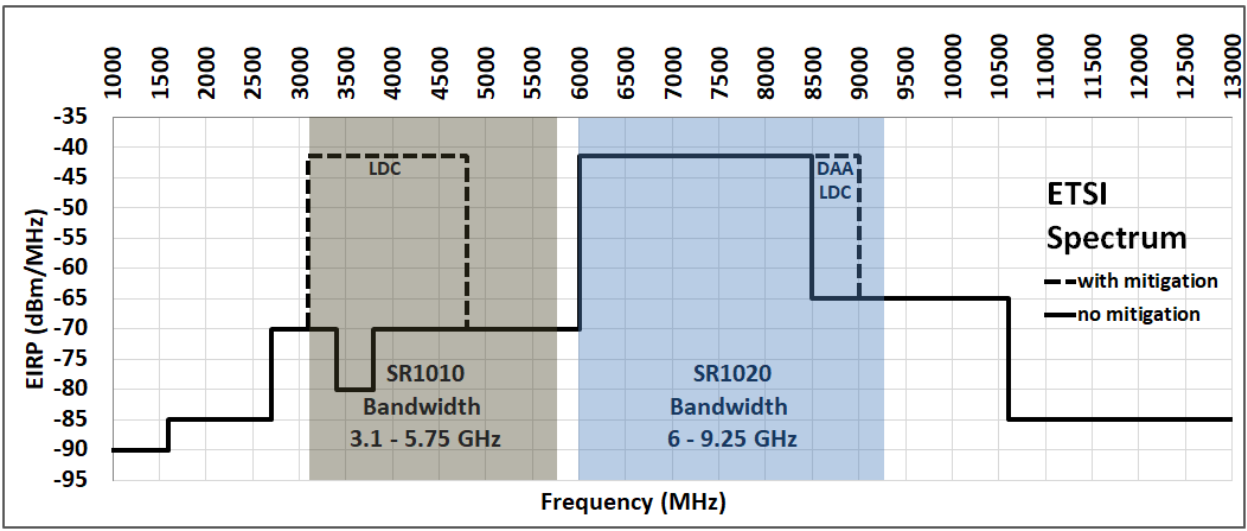
\includegraphics[width=\textwidth]{images/FCC spectrum ETSI.png}
        \caption{Maximum mean emission levels for UWB communications devices by ETSI.}
        \label{fig:spark_ETSI}
    \end{subfigure}
    \hfill
    \centering
    \begin{subfigure}[b]{.49\textwidth}
        \centering
        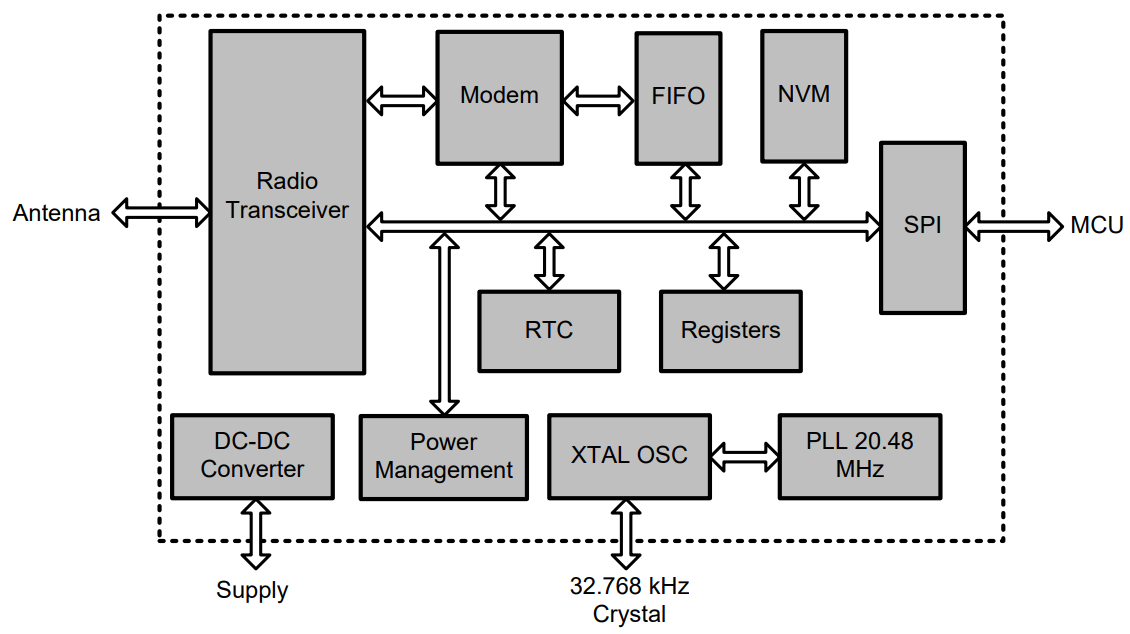
\includegraphics[width=\textwidth]{images/radio picture datasheet.png}
        \caption{System Block Diagram}
        \label{fig:system_block_diagram}
    \end{subfigure}
    \hfill
    \begin{subfigure}[b]{.7\textwidth}
        \centering
        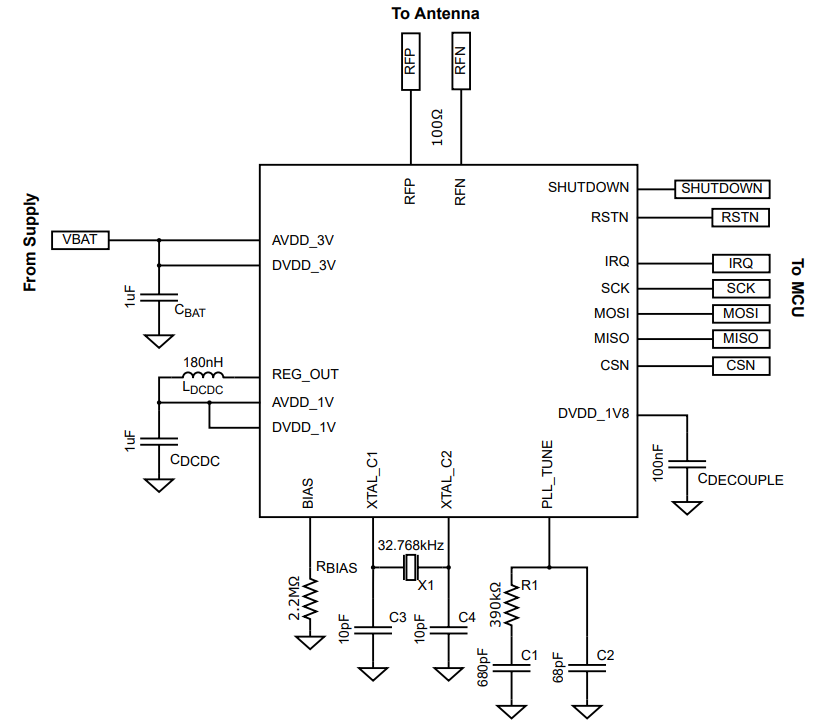
\includegraphics[width=\textwidth]{images/radio circuit datasheet.png}
        \caption{Spark SR1020 Circuit.}
        \label{fig:radio_circuit}
    \end{subfigure}
    \caption{SR1020 Radios Circuit}
    \label{fig:sr1020_radios}
\end{figure}


%2 [depending on the country, I will address this later on].
By using SPARK Microsystems' cutting-edge technology, developers and industries can harness the power of ultra-low latency and energy-efficient wireless communications, opening new avenues in IoT applications and more.

\section{Hardware}
\label{sec:spark_hardware}
This section provides an overview of the radios' hardware specifics and the family evaluation kit employed for characterization. Additionally, I will highlight the topics to be discussed in the characterization chapter and share brief insights into some features.


\subsection{Radios}
When it comes to Bandwidth and Spectrum Configuration, these transceivers have a dynamic UWB spectrum with up to 3 GHz of bandwidth. The SR1010 functions in the 3.1 – 5.75 GHz band, whereas the SR1020 operates in the 6 – 9.25 GHz range. For our analysis, we focused on the SR1020.

Key features include ultra-short latency of 50 µs for a 1 kb airtime and data rates reaching 20.48 Mbps. Detailed discussions on latency and data rates are available in Christian Sassi’s dissertation; I did not partake in those specific characterizations.

What distinguishes the SR1010/SR1020 from other UWB radios is their exceptional energy efficiency. They require just 0.25 nJ/bit to transmit and 1.15 nJ/bit to receive, significantly reducing operational costs. Furthermore, they have adaptable sleep modes: the 'idle' mode (turns off only the radio) and two deeper sleep modes – 'hibernate' and 'deep sleep', which consume 55 nA and 750 nA, respectively. I will delve into this further in the characterization chapter.

Another highlight is their ability to coexist with BLE/WiFi (2.4 \& 5 GHz) and cellular systems, avoiding interference.

Additionally, the SR1000 series, which includes the SR1010/SR1020, can gauge accurate distances between two SPARK chips due to their unique ultra-low power time-of-flight (ToF) measurement system. This ensures roughly 30 cm precision for distances from 0.5 m to 100 m. To provide context, the DecaWave DW1000 offers a slightly better accuracy of +-10 cm\cite{DW1000_manual}. Neither Christian nor I evaluated this ranging accuracy. During our tests, the SDK v1.1.0 lacked the Ranging Core. The latest SDK v1.2.0 was released on 31 May 2023.



The SR1010/SR1020 boasts an architecture that includes a UWB RF transmitter and receiver, a dedicated power management unit, a sleep counter, digital baseband hardware, timers, and a regulator. Its design allows for easy integration with microcontrollers via an SPI interface, which enhances battery longevity in systems. Refer to Figure 3.1 b and c for the radio's system block diagram and circuit, respectively.
	
\subsection{Evaluation Kits}		
For our study, we utilized the Family Evaluation Kits (EVK), specifically the EVK 1.4 which features the SR1020. The EVK's components are illustrated in Figure 3.2. Intended to highlight the radios' capabilities, the SDK Board Support Package (BSP) supports the EVK. For those looking to pair the SDK with a custom board using the SR10X0, Spark provides a porting guide within their SDK documentation, offering valuable insights for optimal performance.


\begin{figure}[h]
\centering
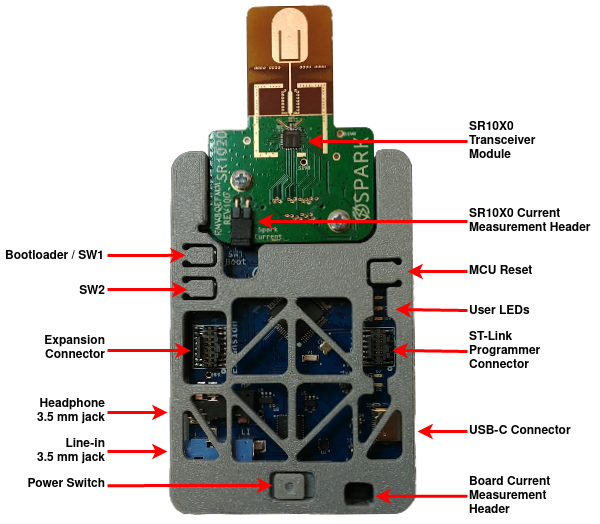
\includegraphics[width=0.7\textwidth]{images/evk picture.png}
\caption{Spark Family Evaluation Kit.}
\label{fig:spark_evk}
\end{figure}

%[Hardware Description — SPARK Microsystems SDK]
The EVK is also equipped with an audio codec and dual 3.5 mm audio jacks. While I won't discuss the EVK and radios in an audio setting, Christian Sassi evaluated the radios' latency within a haptic musical framework. The microcontroller in our EVK was the STM32G474RET6, powered by the Arm Cortex M4 32-bit RISC Core. Although it's capable of running at 170 MHz / 213 DMIPS, it offers multiple low-power modes.
% Add ref to st website
As can be noted, the EVK presents some current probes to measure electrical current. The top-left probe measures the radio's current consumption, while the bottom-right one measures the entire board's consumption - including the radio, microcontroller, codec, and interconnected PCB components.  I employed these measurement headers, paired with a power profiler, to discern their power consumption, details of which will be further discussed in the characterization chapter. Additionally, there's a JTAG expansion connector for peripherals. Via the expansion connector, it is possible to connect UART and SPI sensors. My use of the JTAG connector was limited to debugging, specifically for gauging wake-up delays by sending signals based on internal events.

\section{SDK}
\label{sec:spark_sdk}
SPARK's Software Development Kit (SDK) provides an array of development tools and sample applications. Designed to work hand-in-hand with the SPARK Evaluation Kit (EVK), the SDK equips users with clear application examples, showcasing SPARK's key libraries. It encompasses nearly all SDK features, and a board support package (BSP) further aids in testing these examples on the EVK, facilitating experimentation with SPARK's technology.
When transitioning to custom PCBs, users can adapt the provided samples, using the BSP as a reference throughout the SDK porting phase. The SDK also offers comprehensive guidelines on designing a board with their radios from the ground up. %[FOOTER NOTE TO THE SECTION OF THE WEBSITE]
The SDK encompasses three cores: Audio, Wireless, and Ranging. While Christian and I will address the Wireless Core in our characterization chapters, with a focus on different facets, only Christian delves into the Audio Core. Given the depth of the Wireless Core, I will highlight its salient aspects and features for an easier transition into the subsequent characterization chapter. For more in-depth details, refer to the SDK documentation's Wireless Core section.

% Add ref to the doc


\subsection{Transmission}

\subsubsection{Time Division Multiple Access}
The Wireless Core incorporates a network stack utilizing Time Division Multiple Access (TDMA). Adhering to the TDMA schedule is mandatory for sending packets. TDMA segments time into specific timeslots designated to certain events on every board, enhancing power efficiency. Radios can remain dormant except during their designated transmission timeslots, leveraging the more profound sleep modes available.


\subsubsection{Frequency Switching and Networks of Nodes}
Transmission channels can be altered or cycled through a predetermined list known as a channel sequence – a method known as frequency switching. This optimizes spectrum usage and ensures adherence to the FCC's regulatory emission limits. Creating a network of nodes is straightforward, with some topologies, such as the star network, being readily available. The PAN ID and node addresses facilitate this by establishing logical networks and determining packet recipients. Similar to other technologies, broadcasting packets to nodes under the same PAN is feasible.


\subsubsection{Modulation}
Two modulation types are available: Inverted On-Off Keying (IOOK) and 2-bit Pulse Modulation (2-bit PPM). While IOOK is an amplitude coding that sends a signal for a 0 bit and remains silent for a 1 bit, 2-bit PPM encodes two bits in four signals. Figure 3.3 illustrates their operation.

\begin{figure}[h]
\centering
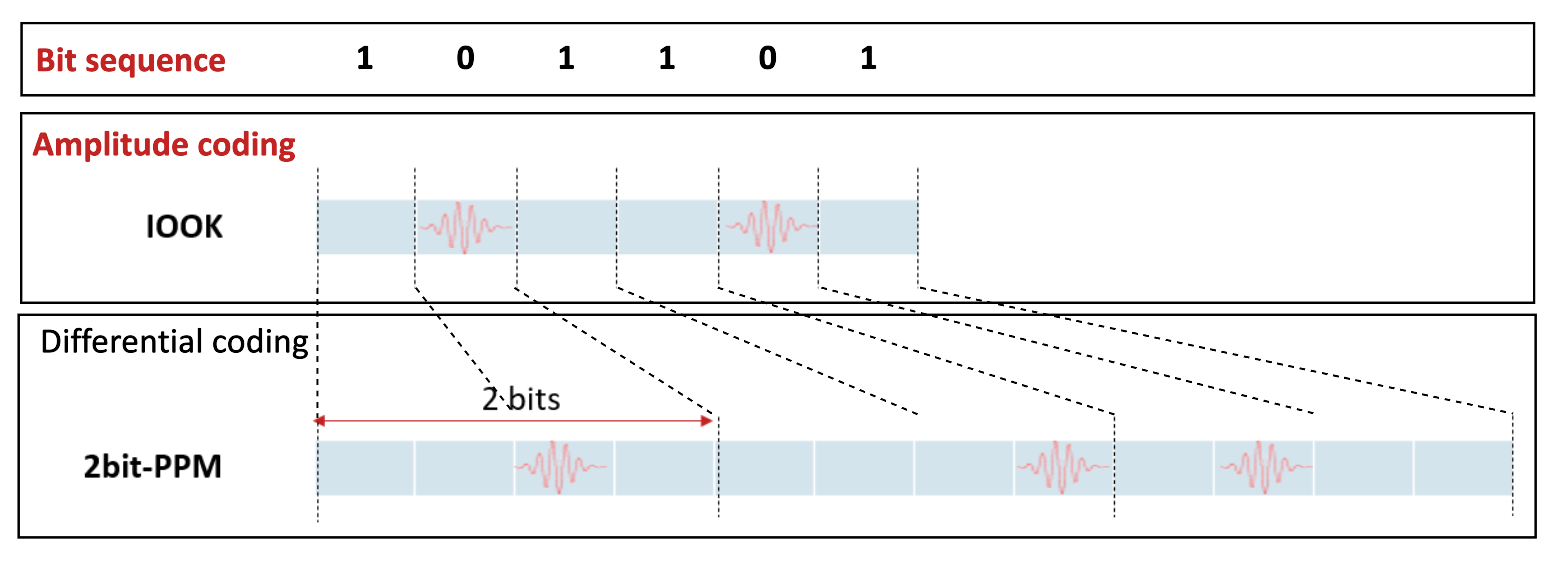
\includegraphics[width=0.7\textwidth]{images/modulation_bit_sequence.png}
\caption{Modulation Bit Sequence.}
\label{fig:modulation_bit_sequence}
\end{figure}

IOOK sends a signal when the bit is 0 and does not send anything when it is 1. Every bit is an impulse, therefore, it enables high data rates. 2bit-PPM sends four signals every two bits. As can be seen in the example in Figure 3.3, the bit sequence of six bits is divided into three blocks of four bits. Every block encodes the pair of bits.

Our characterization favored 2-bit PPM over IOOK, reserving the latter exclusively for high data rate applications.

\subsubsection{Forward Error Correction}
The system offers four distinct Forward Error Correction (FEC) levels. These non-standard levels have been detailed in the subsequent table.

\begin{table}[htbp]
\centering
\begin{tabular}{|c|c|}
\hline
FEC Level & Frame Inflation Rate \\
\hline
0 & x1 \\
\hline
1 & x1.334 \\
\hline
2 & x1.667 \\
\hline
3 & x2 \\
\hline
\end{tabular}
\caption{FEC Level versus Frame Inflation Rate} % Optional: If you want a caption for your table
\end{table}

\subsubsection{Frame Transmission}
A "Stop and Wait" mechanism exists for resending unacknowledged frames. We omitted this in our characterization to assess the packet reception rate without multiple sends.


\subsection{Sleep Modes}
The radios support three sleep modes: Idle, Shallow, and Deep. The deeper the mode, the fewer active peripherals, leading to minimized energy consumption at the cost of increased wake-up delays. A complete radio shutdown labeled the "Shutdown power state", is also available. Further insights will be shared in the characterization chapter.

\subsection{Additional Information}
The Wireless Core and its API are intricate, featuring advanced capabilities not covered here. For instance, the SDK supports fragmenting large frames, a feature employed during my distributed AEP test when the payload exceeded the 125-byte limit. Additionally, there's an "alternative channel configuration" for challenging environmental conditions and a "link throttling" feature to limit throughput and power consumption as required. While numerous other features exist, they fall outside the scope of this dissertation.

\newpage




      \chapter{Spark SR1020 Characterization}
\label{cha:characterization}

\section{Introduction}
In this chapter, I will delineate the tests conducted on the Spark SR1020. Initially, I will present the experiments jointly undertaken with Christian Sassi, highlighting personal observations and derived conclusions. Subsequently, I will emphasize the tests specifically targeting power consumption metrics. The objective is to elucidate the methodologies, outcomes, challenges, and findings without revisiting the details already covered in Christian Sassi's dissertation.

\section{Setup and Environment}
All experiments were performed under consistent environmental conditions, ensuring the reliability and reproducibility of results across various settings of the Wireless Core. We strategically elevated the Evaluation Kits (EVKs) using wooden poles to a height of 145 cm to mitigate potential signal reflection from the floor, which could adversely affect performance metrics. The chosen venue for these tests was the West corridor within the Povo 2 building at the University of Trento. This university is renowned for hosting the extensive CLOVES IoT Testbed, a dedicated facility for Ultra-Wideband (UWB) experiments\cite{CLOVES_website}. To minimize external interference, we ensured exclusive access to the testbed and deactivated all other transceivers. However, it's worth noting that certain environmental factors, such as a specific locker's proximity, had a discernible impact on our measurements. The accompanying image illustrates our experimental setup, especially emphasizing the scenario where the receiver board, termed the ‘node’, was adjacent to the aforementioned locker. All conducted tests adhered to a Line Of Sight (LOS) transmission principle.

\begin{figure}[h]
\centering
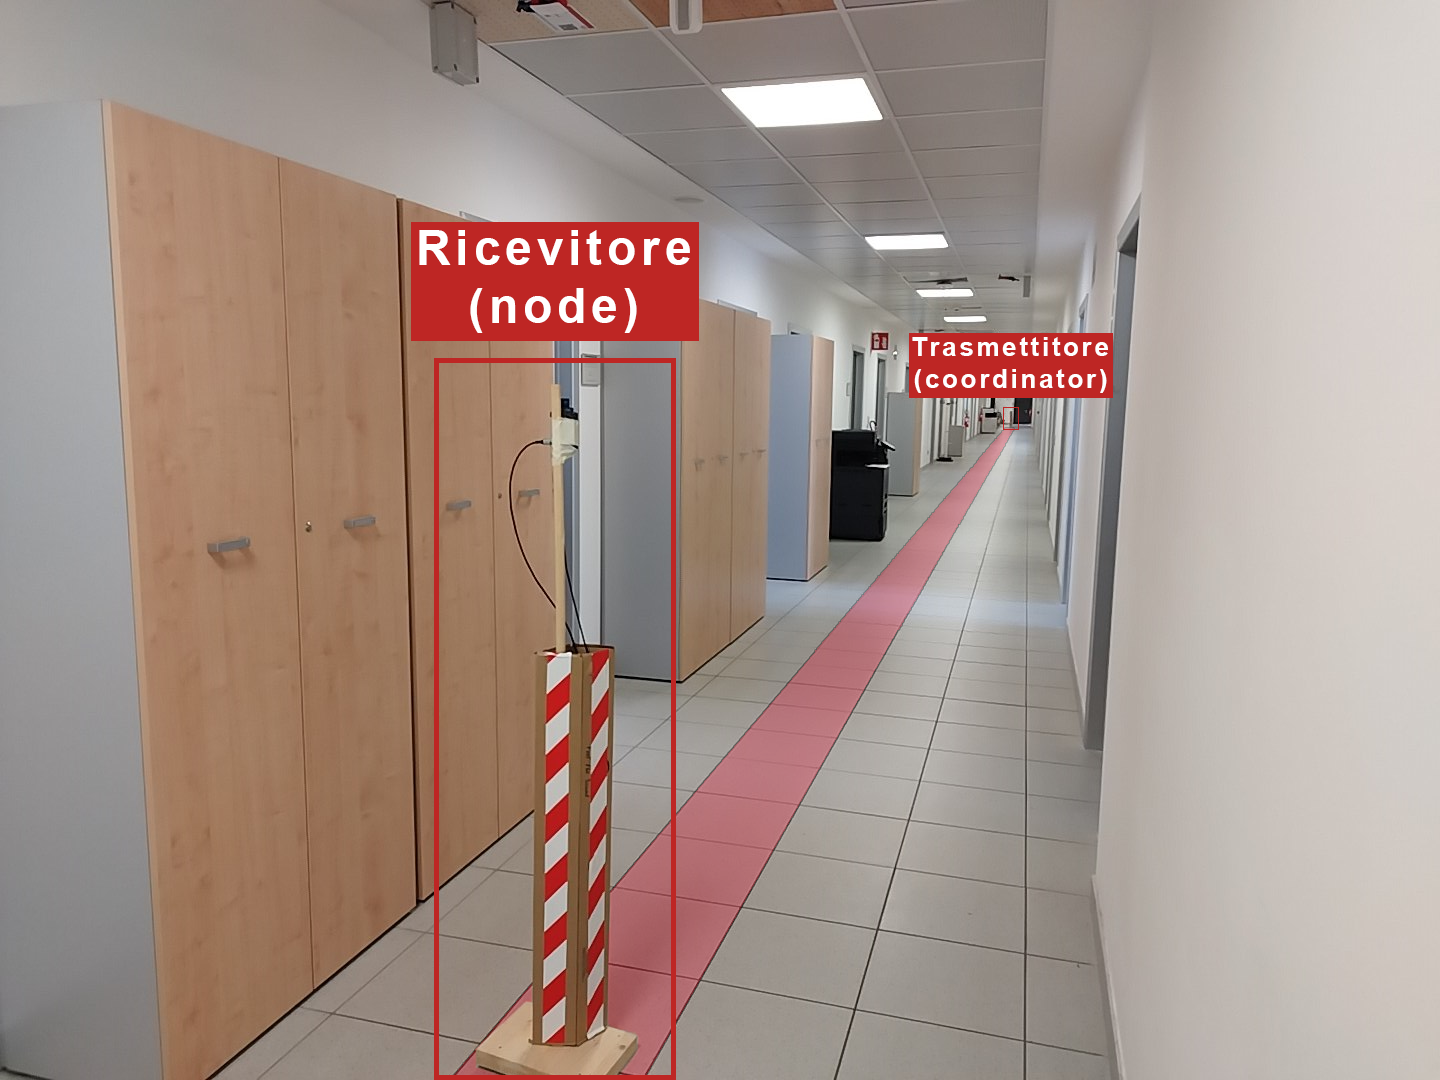
\includegraphics[width=0.8\textwidth]{images/setup test.png}
\caption{Testing Environment}
\label{fig:testing_environment}
\end{figure}

\section{Tests}
Consistency was maintained by employing two distinct boards, designated as ‘node’ and ‘coordinator’ in accordance with Spark's official documentation. Both were configured to execute identical operations. While the 'node' was mobile during tests, the 'coordinator' remained static, serving as our primary connection point. Despite our singular connection to the coordinator, comprehensive statistics for both boards were readily accessible. Given the inherent TDMA-based operation of the Wireless Core, transmissions were scheduled via predefined timeslots. Our experimental paradigm utilized two symmetrical timeslots, each 500 µs in duration, translating to a packet transmission every 1 ms. Features that could potentially introduce variability or unpredictability, such as ARQ, were deliberately disabled. However, we retained the acknowledgment system to effectively monitor the integrity of transmissions.

\subsection{Range Capabilities}
For clarity and precision, I've elected to present only the most robust and pertinent data we amassed. These data points have been consolidated into a single graph presented below. Prior to unpacking the details—especially the noticeable gaps in the 6.5 GHz dataset and the underwhelming performance of the board at this frequency—it's essential to provide context for the data. 
The term 'Coordinator' success rate delineates the Packet Reception Rate (PRR) associated with transmissions originating from the coordinator and directed towards the node. Conversely, the 'Node' success rate signifies the PRR of packets sent by the node to the coordinator. Capturing data from both sources offered deeper insights into the reciprocal transmission behaviors between the radios.
A key observation point was at the 70 m mark, which corresponded to the corridor's terminus, preceding a petite lobby at an intersection of hallways. Tests conducted at 80 m required one board to be placed adjacent to the aisle's terminating wall. This position, within a relatively open expanse, witnessed an uptick in packet reception rates. It is postulated that the wall potentially served as a reflector, enhancing packet reachability to the node. The parameters for these experiments included the Forward Error Correction (FEC) being adjusted to its most minimal setting. This choice was to authentically evaluate range capabilities devoid of augmented payload, which might inadvertently skew power consumption data—a facet I'll explore subsequently.

\begin{figure}[h]
\centering
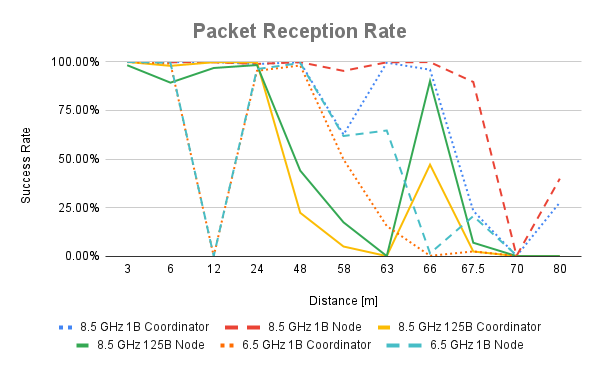
\includegraphics[width=\textwidth]{images/Packet Reception Rate.png}
\caption{Packet Reception Rate}
\label{fig:packet_reception_rate}
\end{figure}


Pivoting to our endeavors at the 6.5 GHz frequency, the results were unfortunately marred by challenges, precluding a full suite of tests akin to the 8.5 GHz frequency trials. Preliminary findings intimate suboptimal performance of radios when operating below 7 GHz, struggling with a limited 6-12 meter range even in ideal conditions. Dedicated tests were carried out to decipher this anomaly. The subsequent graph juxtaposes the success rate in relation to the channel frequency, holding all other variables and the testing environment constant.

\begin{figure}[h]
\centering
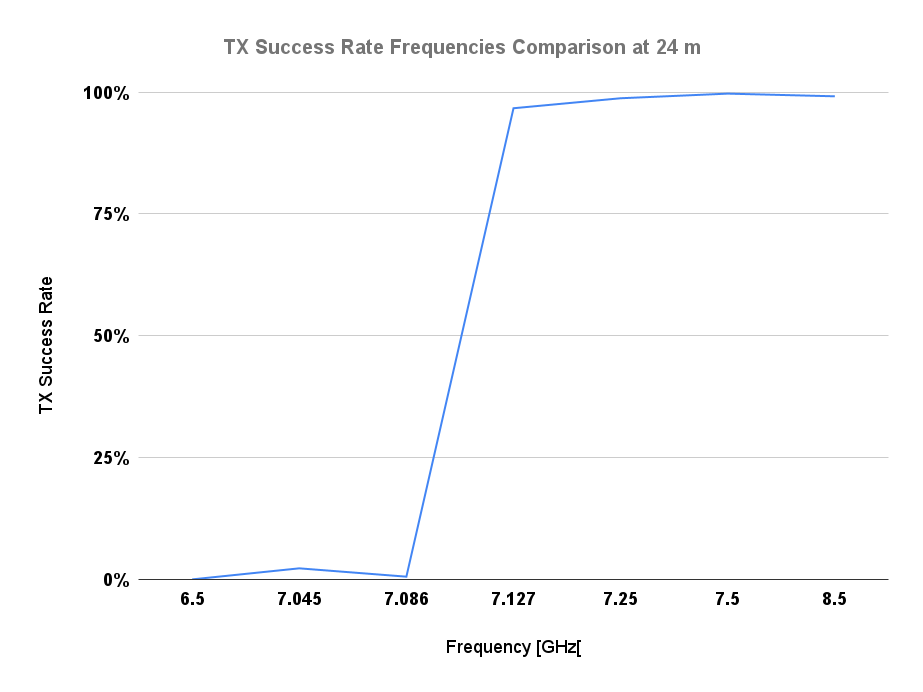
\includegraphics[width=1\textwidth]{images/TX Success Rate Frequencies Comparison at 24 m1.png}
\caption{TX Success Rate Frequency Comparison}
\label{fig:prr_frequency_comparison}
\end{figure}

In the course of my investigation into the underlying causes, I delved into the intricacies of the SDK. Regrettably, due to the lack of support from Spark, I was unable to derive a comprehensive understanding of the phenomena at play. One plausible hypothesis I've formulated is based on Spark's primary application of these radios. Spark predominantly employs these radios for wireless gaming peripherals, encompassing extended reality (XR), headsets, and various gaming devices. Consequently, Spark might have optimized these radios predominantly for short-range scenarios characteristic of such devices.

Subsequent tests were conducted with the Forward Error Correction (FEC) adjusted to the second level. Despite the elevation in the inflation rate to x1.667, the radios exhibited a markedly enhanced performance. Presented below are graphical representations depicting this improved performance and juxtaposing the outcomes from two distinct FEC settings. Additionally, preliminary tests were undertaken with the FEC calibrated to its maximal setting, characterized by an inflation rate of x2. Notwithstanding a marginal improvement in the Packet Reception Rate (PRR), the pronounced inflation rate deleteriously impacted both power consumption and data rate. Hence, our experimental protocol settled on utilizing the second FEC level.

\begin{figure}[h]
\centering
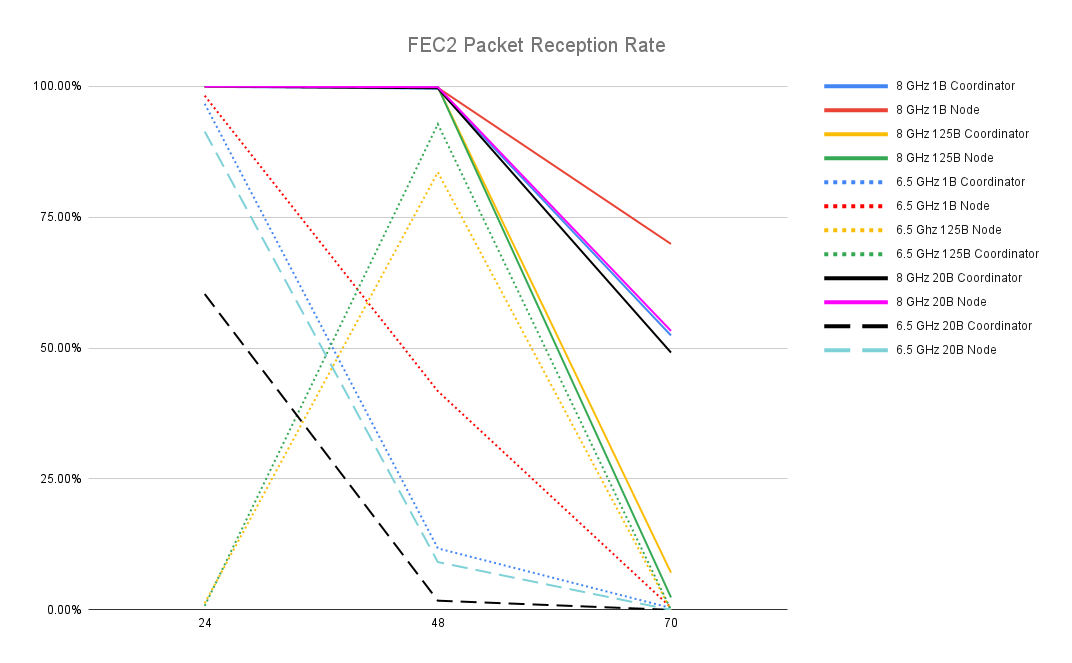
\includegraphics[width=\textwidth]{images/FEC2 Packet Reception Rate.png}
\caption{FEC2 Packet Reception Rate}
\label{fig:fec2_prr}
\end{figure}

A perplexing observation surfaced at the 24m range with FEC 2 and 6.5 GHz: the radios consistently failed to receive any packets. This anomalous behavior persisted across repeated tests, executed at varied intervals and on different days. Notwithstanding our meticulous efforts to mitigate potential interference, the outcome defied our anticipations.

To provide a lucid comparative overview, the subsequent graph delineates the disparity between the two FEC levels. To streamline this representation and given the congruence of the results, only the Coordinator PRR has been plotted, its data being virtually indistinguishable from that of the Node.


\begin{figure}[h]
\centering
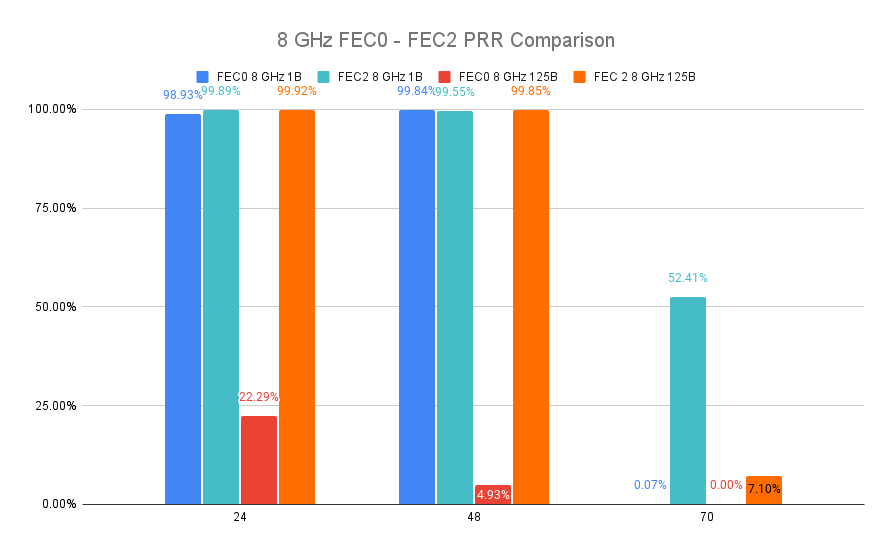
\includegraphics[width=\textwidth]{images/8 GHz FEC0 - FEC2 PRR Comparison.png}
\caption{FEC0 and FEC2 PRR Comparison}
\label{fig:fec0_fec2_comparison}
\end{figure}

\subsection{Power Consumption}
As I will explain in the Challenge chapter, it was infeasible to collect accurate values of power consumption and wake-up timings. I, therefore, decided to report only the data I am confident is correct as I was able to double-check it with different measurement tools. I used the Nordic Semiconductor Power Profiler Kit II (PPK2) and the Diligent Analog Discovery 2. I estimated both metrics based on the data collected and it aligns with what Spark stated. Therefore, I believe that even if for the range capabilities we had some discrepancies between the datasheet and the test results, for what concerns these experiments we did not have many surprises. Figure 3.6 is a Pivot Table that shows the power consumption of the radios using the Idle sleep mode when not communicating.

\begin{figure}[h]
\centering
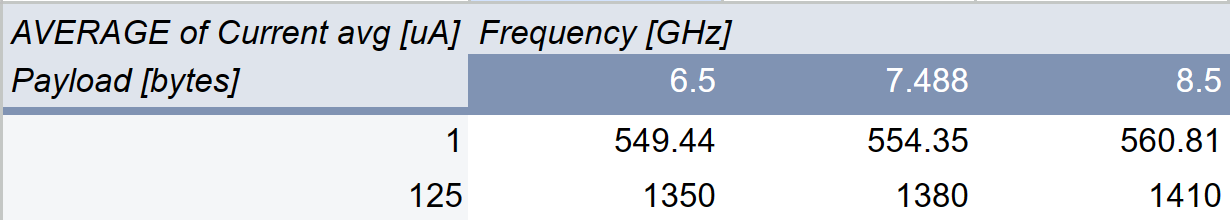
\includegraphics[width=0.8\textwidth]{images/power consumption.png}
\caption{Average Current Pivot Table}
\label{fig:avg_current_pivot}
\end{figure}

Depicted in Figure 4.6 is the average current consumption predicated on the previously described TDMA schedule. A consistent transmission peak, averaging 3.275 mA, was observed throughout the tests. When considering the operational voltage of the radio at 1.8v, its power consumption is discernibly lower, nearly by a factor of ten, when juxtaposed with the DecaWave DW1000, an Ultra-Wideband radio that is in prolific use. This same radio model is also integrated into the University of Trento’s testbed, as discussed in the Setup and Environment section.
%[https://forum.qorvo.com/t/dw1000-power-consumption/10583]

I endeavored to ascertain the delay associated with the wake-up time of all available sleep modes. This necessitated the transmission of impulses via the JTAG expansion connector concurrent with specific occurrences within the event-driven finite state machine intrinsic to the SDK's lower levels. In a corroborative measure, I reduced the TDMA schedule's timeslot duration progressively until the PRR plummeted to 0\%. This strategy aimed at gaining insights into the radio's wake-up latency. Notably, the delays I registered exceeded Spark's official declarations. However, given the methodologies employed, there may have been unavoidable internal delays, thus introducing potential inaccuracies. Figure 4.7 delineates the power states, indicating which devices are active or inactive in each state, accompanied by the respective current usage and wake-up delays.

\begin{figure}[h]
\centering
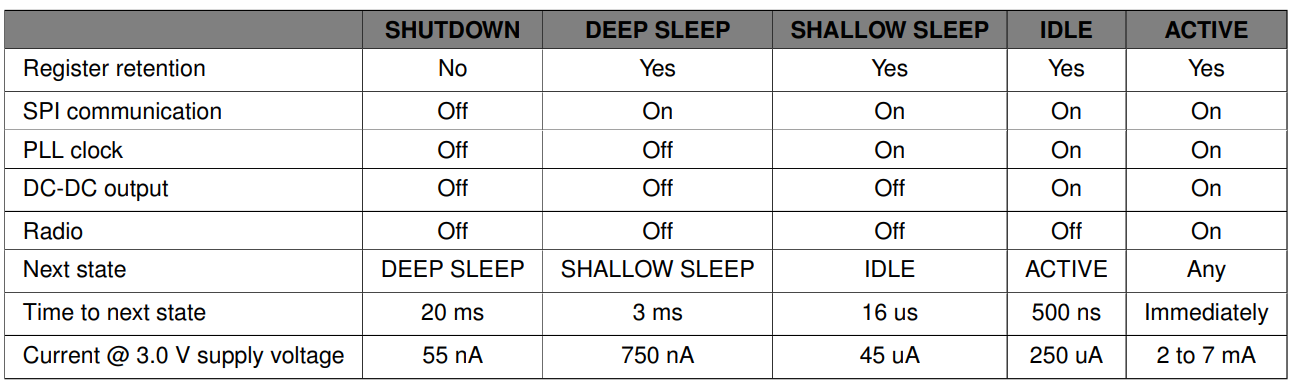
\includegraphics[width=\textwidth]{images/power states datasheet.png}
\caption{SR1020 Power States}
\label{fig:power_states}
\end{figure}


\section{Challenges}
\subsection{Statistics APIs}
Within the Wireless Core architecture, there exists a suite termed 'statistics APIs', dedicated to data extraction from the employed connections. Regrettably, not all the specified functions are fully realized or operational as anticipated. Certain functions, instead of returning values directly, appear to rely on other lower-level functions to update specific structures; this frequently results in absent or incorrect updates. An in-depth probe revealed vestigial functions and structures, possibly remnants from earlier SDK iterations, thus culminating in functional aberrations. Although I managed to retrieve additional values beyond those illustrated in the SDK examples, they fell short of expectations. Consequently, there exists a paucity of data on nuanced metrics such as link quality. However, metrics like RSSI (Received Signal Strength Indicator) and RNSI (Received Noise Strength Indicator) were retrievable. These assisted in demystifying the suboptimal performance of radios at frequencies below 7 GHz. Intriguingly, occasional readings for both metrics registered 0 dB — while conceivable for the RSSI, it's improbable for RNSI due to the ever-present noise factor. Given these inconsistencies, such values were excluded from the characterization.

\subsubsection{Serial Communication}
Data transmission to the boards via serial proved insurmountable despite the presence of relevant functions and the appropriate utilization of the HAL (Hardware Abstraction Layer) within the SDK. Engaging with Spark on this challenge yielded the revelation that this capability has not been extended to the Evaluation Kits. The rationale behind this unilateral serial transmission remains enigmatic to us, but it undeniably curtailed our ability to optimize test execution through automation.

\subsection{Accurate Power Consumption Measurement}
In an effort to derive precise data on power consumption, it became evident that the power profilers utilized were not adept at discerning the distinct stages of the transceivers, such as wake-up, transmission, synchronization, and so forth. When an attempt was made to integrate a shunt resistor between the designated current measurement header pins, an unintended diversion of current was observed, ostensibly from an alternative component of the circuit. This rendered oscilloscope-based measurements impractical.

When a minimal resistance was incorporated for current measurement related to the radio, the oscilloscope predominantly displayed electrical noise. Conversely, slightly increasing this resistance resulted in the current bypassing our intended path and instead traversing another section of the PCB, which left the resistor devoid of any current. Incremental adjustments, even by a single Ohm, failed to produce a satisfactory measurement condition. Notably, this appears to be a slight oversight in the PCB design. Interestingly, this investigative process illuminated the fact that the radios maintained functionality even when the current measurement header pins were entirely disengaged, drawing current entirely from alternative pins. This anomaly was closely studied in collaboration with Davide Molteni, a technician affiliated with the Department of Information Engineering and Computer Science. Our consensus posits that the radio might be sourcing its current through the CS (Chip Select) pin associated with the SPI interface.

From a theoretical standpoint, the optimal approach to executing these tests without altering the hardware might entail employing a sophisticated oscilloscope, equipped with an efficient probe and a shunt positioned between the current measurement pins. Nevertheless, the plausibility of this method remains ambiguous, given the challenges posed by potentially negligible voltage levels susceptible to noise interference. In the event of this approach being untenable, two viable alternatives emerge:

\begin{enumerate}
  \item Extracting the radio from the EVK and subsequently engineering a breakout board that effectively connects the two. This setup would incorporate test pads, current measurement pin headers, and jumper connections across all pins bridging the two PCBs. This configuration promises enhanced insight into the current distribution across the various radio pins.
  \item Rethinking the radio PCB's design from its foundational stage. Commencing with solely the SR10X0 chip and adhering to the hardware design guidelines could prevent such inadvertent current flow patterns. 
\end{enumerate}


%[ADD LINK TO WEB PAGE]

\newpage





      \chapter{Distributed AEP}

\section{Self-learning Autonomous Edge Learning and Inferencing Pipeline (AEP)}
\label{AEP}
The Autonomous Edge Learning and Inferencing Pipeline (AEP) is an innovative approach designed to harness the potential of unsupervised learning in IoT environments. At its core, the AEP consists of two main stages:
\begin{enumerate}
    \item Pseudo-label Generation, using the k-means++ clustering technique, intelligently groups unlabeled data.
    \item Local Training and Classification, where once pseudo-labels are assigned, the AEP engages in the training process with either the decision tree (DT) or the k-nearest neighbor (k-NN) classifiers.
\end{enumerate}

This system stands out particularly for its adaptability in resource-constrained scenarios, ensuring efficient on-device ML operations. The creation of AEP comes in response to the challenge of managing vast amounts of unlabeled data generated by IoT devices, pushing the boundaries of traditional supervised learning models. Its design prioritizes flexibility and robustness, making it suitable for various microcontrollers and edge devices. It achieves robustness thanks to its sample filtering, used to delete outliers. Moreover, it can cope with the constant inflow of data with memory overflow control techniques, using FIFO, RND, and CONF memory filtering. FIFO (First In First Out) prioritizes new data over old data. When the memory is full, the oldest samples are deleted to accommodate the newest ones. RND, instead, randomly selects some samples to delete. CONF selects the data points to delete based on their confidence level. The confidence level measures how likely a data point is valuable. Euclidean distance measures how close the sample is to the kmeans++ centroids. There are also three parameters for the memory management of the pipeline. The memory size indicates how many samples we want to be saved at any time. The initial threshold and the update threshold are used to decide how the pipeline behaves. The initial threshold is the starting memory size, which is then increased by increments of magnitude update threshold until reaching the memory size. When the memory is full, the incoming data are accepted by freeing memory with the methodologies stated above. In the paper, there are also efficiency tests and many considerations on memory and CPU usage. I will not delve into such details since I only use the AEP as a starting point for my DML approach. I have modified the AEP to better fit the goal of distributing it albeit preserving its memory-constrained and power-efficiency characteristics. How I modified it and why will be discussed in the Distributed AEP chapter.
% Remember to add the ref to the paper


\label{cha:distributed_aep}
The primary objective of this study was to decentralize the autonomous edge learning and inferencing pipeline (AEP), across a network of low-power nodes. The challenge lies in enhancing the inference accuracy without incurring significant data communication overheads or computational burdens. The starting point for this endeavor was an existing AEP, the source code for which was publicly accessible on GitHub; readers can find the repository link within the associated paper. The subsequent sections detail the modifications made to tailor the pipeline to the outlined scenario, followed by an overview of simulation processes implemented in Python. The final implementation, encompassing the system design and algorithm for node contribution aggregation, was not without its challenges, discussed comprehensively in the System Implementation section. For verification purposes, one of the two datasets used by the original AEP creators was employed, specifically the Pima Indians Diabetes Database\cite{diabetes_db}, intended for diabetes detection. The second dataset, related to semiconductor manufacturing process anomalies, was not chosen due to its already high inference accuracy achieved by the original AEP. With the Pima database, the initial accuracy was approximately 70\%, offering potential avenues for enhancement.

% Add reference to database

\section{AEP Modification}
\label{sec:aep_modification}

The AEP required only minor modifications. With an intent to deploy the k-NN algorithm, the decision tree components and its associated dependencies were excised. Significant changes were made in terms of output presentation: the initial output—a simple summary of pipeline settings, k-means++ centroid coordinates, and post-testing phase accuracy—was transitioned to a JSON format to facilitate subsequent simulations. Furthermore, the k-NN algorithm was enhanced to include additional information in the JSON output, such as coordinates of the nearest neighbors, their respective scores, and labels. The score for each neighbor, essentially a confidence metric, is integral to the k-NN algorithm; it is utilized to rank the neighbors before selecting the top k entries. This score is determined by the inverse of the Euclidean distance relative to the centroid coordinates. To augment the AEP's adaptability, several macros were incorporated.

Although the existing pipeline demonstrated a degree of flexibility, the intention to simulate a plethora of settings combinations in Python necessitated the introduction of more macros to adjust its operational behavior. Table 5.1 enumerates the most crucial macros that were integrated for pipeline configuration.

\begin{table}[]
\centering
\caption{Macro Definitions}
\begin{tabularx}{\textwidth}{lX}
\toprule
\textbf{Macro}          & \textbf{Meaning} \\
\midrule
SIMULATION              & Enables simulation mode (deletes previous macro definitions) \\
N\_NODES / NODE\_ID     & Number of nodes, and current node id \\
K\_NEIGHBOR             & Number of neighbors for the k-NN \\
MEMORY\_SIZE            & Maximum data points stored at once \\
CONFIDENCE\_THR         & Confidence threshold for k-means++ \\
FILTER                  & Filter to apply to discard samples (CONF, FIFO, RND) \\
ONE\_SHOT               & Runs the pipeline only once \\
INITIAL\_THR            & Initial number of samples stored \\
UPDATE\_THR             & Number of samples introduced at each iteration \\
K                       & Number of clusters for k-means++ \\
ITERATION               & Maximum number of iterations for k-means++ \\
\bottomrule
\end{tabularx}
\end{table}


\section{Aggregation Algorithm Design}
\label{sec:aggregation_algorithm}
The aggregation algorithm aims to assimilate minimal data while enhancing inference accuracy through contributions from a node network. I conceptualized three primary aggregation algorithms, with two of them possessing two distinct variants. Given the intention to simulate various pipeline settings, all the algorithmic approaches were implemented, facilitating a comprehensive comparison of their respective performances, strengths, and shortcomings. While a deep dive into the specifics of each algorithm's implementation is beyond the scope of this section, those interested can refer to the GitHub repository linked in the abstract for the source code.

\subsection{Aggregation Only Incorporating Scores}
This approach offers a straightforward method of aggregating node contributions. A brief representation of its core functionality is provided in the ensuing pseudo-code. Notably, as will be evident in the forthcoming simulation segment, this simplistic algorithm's efficacy exceeded initial expectations.

\newpage

\begin{lstlisting}[language=C]
Initialize: empty map called WEIGHTED_VOTES
Set K to the minimum of n_neighbors and 5

FOR i from 0 to K-1 DO
    Set (SCORE, LABEL) to the ith element of SORTED_NEIGHBORS
    IF LABEL is not a key in WEIGHTED_VOTES THEN
        Add LABEL as a key to WEIGHTED_VOTES with a value of 0
    END IF
    Increment the value associated with key LABEL in WEIGHTED_VOTES by SCORE
END FOR

Set PREDICTED_LABEL to the key in WEIGHTED_VOTES with the maximum value
\end{lstlisting}

The advantages of this method are conspicuous: minimal data transmission and rapid aggregation. Averaging a data footprint of 4 bytes per neighbor for each node, this stands as the most resource-efficient algorithm among those evaluated. Additionally, its design eliminates the need for sharing data points, thereby ensuring the privacy of the dataset in use.
The algorithm presented exhibits a relatively modest computational overhead. Initially, it aggregates scores sent by nodes into a singular array, which subsequently requires sorting. The most computation-intensive step here is the sorting process, possessing a complexity of \(O(n)\), where \(n\) is the product of the number of nodes and neighbors. Nevertheless, optimization opportunities exist. By employing a sorted data structure, the computational burden associated with adding each node's contribution could increase, but it ensures that the array remains sorted. Consequently, the computational complexity for this initial phase would be reduced to \(O(\log n)\). However, the algorithm must then iterate through the first \(k\) values, introducing an \(O(k)\) complexity. Therefore, the overall complexity can be described as \(O(\max(\log n, k))\).


\subsection{Aggregation Incorporating Coordinates}
While this strategy demands more data, its execution remains swift. It necessitates coordinates of the centroids, supplemented with neighbor-specific data from all nodes. As alluded to earlier, two variations of this approach exist: one capitalizes on the distance between neighbors and centroids for weighted voting, while the other leverages the distance between neighbors and the test datum. The high-level pseudo-code that follows amalgamates both variants, mirroring the algorithmic implementation used during simulation.  



\begin{lstlisting}[language=C]
Initialize: correctly_classified_counter_test, correctly_classified_counter_centroids
Compute: averaged_centroids using centroids

For each test in y_test:
    Compile all_neighbors_data from neighbors for the test

    Compute distances:
        - Distance from each neighbor to averaged_centroids (distance0 and distance1)
        - Use distance0 and distance1 to compute the new labels
        - Distance from each neighbor to test_coordinates (distance_from_test)

    Store neighbors sorted by distance_from_test and distance_from_centroid

    Calculate label prediction for:
        - Closest neighbors using distance_from_test
        - Closest neighbors using distance_from_centroid

    Update counters for correct predictions

Return: correctly_classified_counter_test, correctly_classified_counter_centroids
\end{lstlisting}

In this scenario, the computational complexity significantly escalates due to the algorithm's requirement for coordinates of both neighbors and centroids from all nodes in the network. Given that the algorithm employs the Euclidean distance, the complexity remains linear with respect to the count of nodes and their neighbors.


\subsection{Aggregation Incorporating Coordinates with Normalization}

This methodology employs the same data input as its predecessor but requires extended computation time due to the inclusion of normalization. Notably, the differential factor between this and the simplistic coordinate-based aggregation is the normalization applied to the coordinate data derived from nodes. As underscored in the foundational chapter, the Euclidean distance metric is inherently susceptible to disparities in feature magnitudes and scales. My choice of normalization was the z-score standardization, a prevalent method in the field. An alternative, the min-max standardization, was also assessed but proved incompatible with the specific data set used in this context.

Z-score standardization recalibrates data values to yield a mean of 0 and a standard deviation of 1, described mathematically as:
\[ z = \frac{x - \mu}{\sigma} \] where \( x \) is the original value, \( \mu \) is the mean of the dataset, and \( \sigma \) is the standard deviation.
This algorithm posed the most intricate implementation challenges. As discussed in the subsequent Simulation chapter, the results were not entirely satisfactory. The key hurdle was determining the appropriate normalization technique. Initial testing phases produced suboptimal prediction accuracy. However, subsequent refinements, which involved employing a neighbor set to derive the mean and standard deviation for data normalization, yielded improvements. This exploration encompassed iterative experimentation, leading me to posit that superior normalization approaches likely exist, though they remain unidentified in this study. Ideally, this algorithm should have outperformed its counterparts; its underwhelming performance can likely be attributed to the normalization data choice.

Mirroring its predecessor, this algorithm also has two variants, outlined in the ensuing high-level pseudo-code.  


\begin{lstlisting}[language=C]
Initialize: correctly_classified_counter_test, correctly_classified_counter_centroids, all_neighbors

Compile all_neighbors from neighbors

Calculate mean_coordinates and std_coordinates of all_neighbors

Normalize centroids using mean_coordinates and std_coordinates to get normalized_centroid

Calculate averaged_centroids from normalized_centroid

Normalize tests_coordinates using mean_coordinates and std_coordinates

For each test in y_test:
    Normalize neighbors for the test
    Compile all_normalized_neighbors from normalized neighbors

    Compute distances for each neighbor:
        - Distance from each neighbor to averaged_centroids
        - Use the distance to averaged_centroids to compute the new labels
        - Distance from each neighbor to normalized test coordinates

    Store neighbors sorted by distances

    Predict label for:
        - Closest neighbors using distance to normalized test coordinates
        - Closest neighbors using distance to centroids

    Update counters for correct predictions

Return: correctly_classified_counter_test, correctly_classified_counter_centroids

\end{lstlisting}

The computational complexity of this algorithm mirrors that of the previous one, though the associated multipliers are considerably larger due to the normalization process. Despite this, the volume of data transmitted remains unchanged from its predecessor. Additionally, the algorithm necessitates supplementary data structures to accommodate the mean and standard deviation of the neighboring data.


\section{Simulation and Results}
\label{sec:simulation}
A suite of Python scripts was developed to simulate a network of nodes, with the details accessible via the accompanying GitHub repository.

The script titled \emph{compilation\_execution.py} serves dual functions. Initially, it enumerates all potential pipeline configurations, transforming them into gcc compilation strings, which are subsequently executed within a shell script. This produces a directory populated with JSON outputs corresponding to each executable. Given the data intensity resulting from this process, it became imperative to focus on configurations that most significantly impacted performance. Thus, the simulation was constrained to a single iteration (under the one-shot setting), with no limitations imposed on k-means++ iterations. Leveraging the one-shot setting meant inherent restrictions on macros related to sample dropping and memory management. This strategic approach culled the total configurations from an overwhelming 94,320 down to a manageable 8,040. These adjustments ensured that the study remained comprehensive, yet efficient without necessitating specialized data structures. Optimized for 16 cores, the script processes the compilations and executions within a span of approximately an hour.

Subsequently, the \emph{aggregate\_all.py} script comes into play, amalgamating JSON files that share identical prefixes. This signifies that while their configurations remain constant, they correspond to different nodes within a single network. Once populated with data extracted from the JSON files, the script initiates the aggregation algorithms, culminating in a comprehensive CSV file. This file juxtaposes the performance metrics of each algorithm against the base accuracy of the pipeline, sans aggregation. This CSV file is structured with fifteen configuration columns, but only five feature the entire spectrum of value combinations, attributed to the previously discussed complexity reduction. Additionally, the file delineates the original accuracy alongside the accuracies derived from the five implemented algorithms. The accuracy assessments utilized the entirety of the test dataset, encompassing 154 data points.

Despite the reduction in complexity, there remained 8,040 possibilities. When nodes were aggregated, this number equates to 2,880 distinct configurations. Representing these results with clarity and succinctness poses a challenge, especially in graphically concise formats. Let's explore the overarching trends in algorithmic performance.

\begin{figure}[h]
\centering
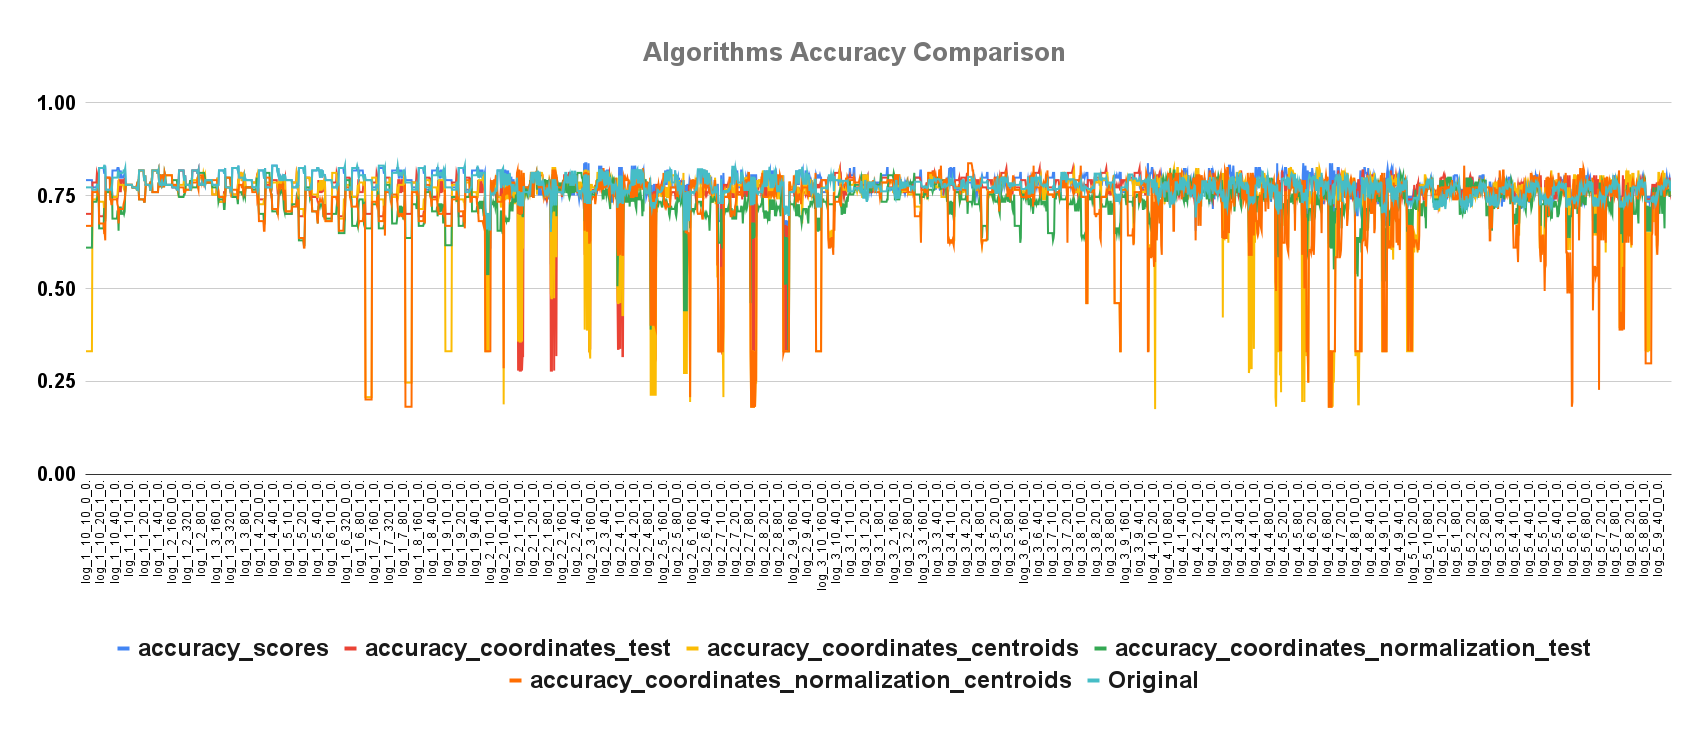
\includegraphics[width=\textwidth]{images/comparison_aggregation_algorithms1.png}
\caption{Comparison Between Aggregation Algorithms}
\label{fig:aggregation_comparison}
\end{figure}

For ease of reference, each algorithm is designated a numerical identifier as illustrated in Table 5.2.

\begin{table}[htbp]
\centering
\begin{tabular}{|c|c|}
\hline
Algorithm & Number \\
\hline
Only scores & 1 \\
\hline
Coordinates, distance to centroid & 2 \\
\hline
Coordinates, distance to test data & 3 \\
\hline
Normalized, distance to centroid & 4 \\
\hline
Normalized, distance to test data & 5 \\
\hline
\end{tabular}
\caption{Association Algorithm - Number}
\end{table}


Figure 5.1 offers a visual comparison of the inference accuracies of all algorithms. The y-axis represents accuracy while the x-axis details possible setting combinations, organized by ascending order based on the number of nodes, memory size, and number of neighbors. Remarkably, the simplest algorithm, algorithm 1, showcased commendable performance, even surpassing the original in specific settings. For configurations with four and five nodes, this algorithm's accuracy paralleled and occasionally outstripped, its more complex counterparts. In settings involving high memory size and five nodes, algorithm 5 stood out with 80\% accuracy in several instances, as opposed to about 70\% of the original one. Yet, algorithm 1 trailed by a mere 2\% and demonstrated greater consistency. The performance of algorithms 2 through 5 varied considerably with specific settings, ranging from an average of 79\% down to a nadir of 17.53\% for algorithm 2. Notably, algorithm 5 never dipped below 33\%. Algorithms 2 and 4, which gauged distances from centroids rather than test data, exhibited lackluster results, averaging a 3\% performance reduction. Their performance variability was also stark, plummeting to 17\% and 18\%, respectively, in contrast to their alternative techniques which maintained a floor of 28\% and 33\%. While algorithm 5 was projected to be the pinnacle of accuracy, its performance was hindered by unresolved issues in certain settings. For comprehensive details, the entire CSV file is accessible on the associated GitHub repository.


\newpage





      \chapter{Conclusions}
\label{cha:conclusions}

The culmination of three years of intensive study, this dissertation illuminates the multi-faceted challenges and potential solutions in the realm of wireless communication with memory-constrained devices. The research journey traversed two primary, interconnected terrains: a meticulous characterization of the Spark SR1020 radios and the pioneering developments in distributed machine learning (DML) tailored for memory-restricted settings.

Through an exhaustive exploration of the Spark SR1020 radios, this study underscored their pivotal role in modern wireless networks. Their distinct attributes, particularly the low-power characteristics, have shown to be indispensable in environments where managing environmental interferences is paramount. This characterization serves not just as a contribution to the field but also as a beacon for future hardware development and optimization.

Transitioning to DML, this dissertation has provided an in-depth examination of existing self-learning ML pipelines, laying a foundation upon which novel algorithms were introduced. The surprising efficacy of the elementary score-based algorithm, in particular, presents both an exciting avenue for further exploration and a testament to the potential of simplicity in design.

Furthermore, the comparative evaluation of various aggregation algorithms and normalization techniques emphasizes the need for continued innovation. While significant strides were made, the field remains ripe for further research and exploration, especially as technological advancements continue to reshape the landscape of wireless communication.

The harmonious convergence of hardware and computational strategies, as demonstrated through the study of the Spark SR1020 radios and DML paradigms, offers a blueprint for navigating the intricate maze of memory constraints and algorithmic innovation. The challenges faced and the solutions proposed herein not only reflect the state of the art but also provide a vision for the future of wireless communication systems.

\section{Future Work}
This dissertation provides an in-depth exploration of two primary domains: the characterization of the Spark SR1020 Ultra-wideband radios and the design and evaluation of Distributed Machine Learning (DML) algorithms for memory-constrained environments. While the findings and methodologies presented herein are the culmination of extensive research, there remains room for further refinement and exploration in both domains.


\begin{enumerate}
    \item Characterization of the Spark SR1020 UWB Radios: The power consumption measurements for the Spark SR1020 UWB radios presented in this dissertation were foundational, yet there's scope for refinement. Given the instrumental constraints during my internship at the University of Trento, the assessments were inherently limited. Future endeavors can focus on employing more sophisticated measurement tools and methodologies to provide a more granular understanding of the power dynamics of these radios.
    \item Distributed Machine Learning Algorithms: The DML algorithms developed and evaluated in this work, while innovative, open avenues for continued research. A particular point of interest is the normalization process integrated into one of the algorithms. Theoretically, this process should bolster the algorithm's performance, positioning it as a superior choice among its counterparts. However, the current implementation doesn't harness its full potential. A more nuanced approach, potentially involving iterative refinements and extensive testing, might be instrumental in optimizing its performance. Given more time and resources, it's plausible to posit that this normalization-centric algorithm can outshine the others presented in this research.
\end{enumerate}


In conclusion, while this dissertation marks a significant step forward in bridging the intricacies of hardware constraints with algorithmic advancements in the realm of wireless communication, the journey is far from over. The insights gained from this research pave the way for deeper explorations, promising further innovations in the confluence of UWB radios and DML paradigms.


\newpage





      
      
    \endgroup


    % bibliography - bibtex format
    %
    % add chapter to index
    \addcontentsline{toc}{chapter}{Bibliography}
    % alphabetical order of authors
    \bibliographystyle{plain}
    \bibliography{biblio}
%%%%%%%%%%%%%%%%%%%%%%%%%%%%%%%%%%%%%%%%%%%%%%%%%%%%%%%%%%%%%%%%%%%%%%%%%%
%%%%%%%%%%%%%%%%%%%%%%%%%%%%%%%%%%%%%%%%%%%%%%%%%%%%%%%%%%%%%%%%%%%%%%%%%%
%% Nota
%%%%%%%%%%%%%%%%%%%%%%%%%%%%%%%%%%%%%%%%%%%%%%%%%%%%%%%%%%%%%%%%%%%%%%%%%%
%% In the bibliography, all the sources consulted for the dissertation 
%% have to be cited and listed in alphabetical order by the 
%% first author's surname.
%%
%% According to the source material, the quotation has to be as follows:
%%
%% BOOKS
%% Surname and initial/s of the name/s of the author/s, date of edition,
%% publishing house and (if applicable) number of edition.
%% 
%% JOURNAL ARTICLES 
%% Surname and initial/s of the first name/s of the author/s,
%% title of the article, name of the journal, volume number, issue number
%% and page numbers.
%% 
%% CONFERENCE PAPERS
%% Surname and initial/s of the name/s of the author/s,
%% year of the conference, title of the article, name of the conference,
%% place of the conference, conference dates, page numbers.
%% 
%% CITING WEB RESOURCES
%% The consulted webpages have to be listed in alphabetical order. 
%% It is necessary to:
%%   - Copy the specific URL (the web address) of the consulted webpage
%%   - If available, indicate the surname and first name of the author/s,
%%     the title and subtitle of the text
%%   - If available, indicate the last date you retrieved the webpage
%%     (day/month/year).   
%%%%%%%%%%%%%%%%%%%%%%%%%%%%%%%%%%%%%%%%%%%%%%%%%%%%%%%%%%%%%%%%%%%%%%%%%%
%%%%%%%%%%%%%%%%%%%%%%%%%%%%%%%%%%%%%%%%%%%%%%%%%%%%%%%%%%%%%%%%%%%%%%%%%%
    

    \titleformat{\chapter}
        {\normalfont\Huge\bfseries}{Appendix \thechapter}{1em}{}
    % Appendix / attachment section - optional
    \appendix
    %\chapter{Title first appendix}



\end{document}
